Even though deep learning has allowed us to do a giant leap forward on the performance of several tasks, and contrary to what some researchers claim \cite{DBLP:journals/corr/KaiserGSVPJU17}, there exists no universal model. A good model would be able to be performant in very different settings, but it won't be able to handle every situation. We need our model to be robust, but we can not expect it to be perfect. Being aware of the limitations intrinsic to the model is the best way to alleviate possible mistakes. Although it sometimes seems the case, deep learning is not a magic box, it learns from the data that we supply. If the model is biased, in all likelihood, it means that our training set is biased. In this chapter, we briefly discuss the details of implementing our method to be used in real-world setting.\\

\section{Final Model}

In the previous chapter, we trained and validated several models. We found that our methodology is quite useful in the task of locating damaged buildings. We now centered our efforts in creating a final model taking into account the entire dataset of 600 tagged samples. This model was not validated as there were no images left to use as a testing set. This process would closely resemble a real pipeline.\\


We used $0.95$ as our decision threshold. According to the best of our models, this threshold guarantees us that we would have around a $0.47$ probability assigning a damaged label when the condition is present while only having a $0.01$ likelihood of mislabeling a no damaged building. While this decision threshold was not necessarily valid for our final model, it gave us a hint on what decisión to make. We are sacrificing sensibility for specificity when we predict a damaged building we are confident that it will be a true positive. We could argue about the low probability of assigning a damaged label, but it all makes sense if we think that we test many samples for each zone.\\


\section{Post-processing}

So far we have centered our discussion on training a model that can categorize images of a particular size. Using such a model to detect collapsed buildings from the drone imagery and geolocating our findings is an entirely different story. We must post-process the information given by the model to transform it into insights.\\

\subsection{Overlapping}

We envisioned two methods to apply our predictive model to a full image. Sliding-window, in which we move a fixed squared along the x-axis and the y-axis, and for each $(x,y)$ value the model is used to predict the condition of the particular window. Another method is to use random sampling, in which we place the window randomly in the image, and then the model is used in the same fashion using a parameter to control the density of the windows. In both cases, we saved the locations of the windows with positive outcome and painted them over the original image. We show an example of our results using the random sampling method in Figure \ref{fig:overlap}.\\

\begin{figure}[!h]
  \centering
  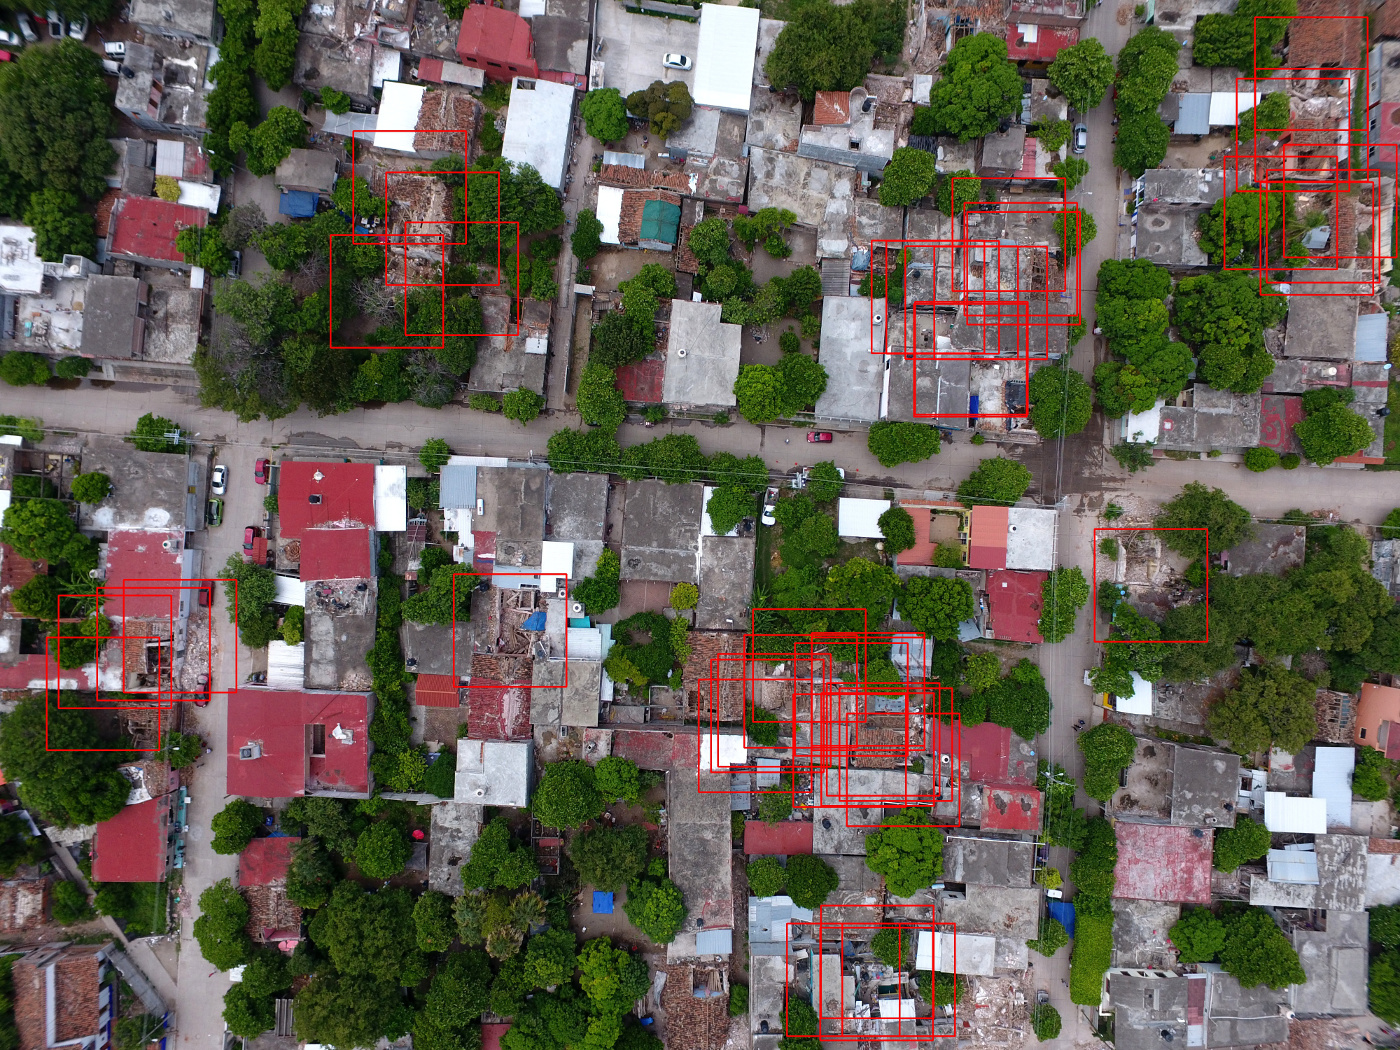
\includegraphics[width=\textwidth]{images/overlap.jpg}
  \label{fig:overlap}
  \caption{Results of our experiment. As we expected, the graph shows a positive correlation between the accuracy and the number of training samples.}
\end{figure}




It is evident that this approach has inherent flaws, as damaged sites are counted several times by the algorithm. A method to alleviate overlapping bounding boxes is known as non-maximum suppression (NMS), a technique borrowed from facial recognition algorithms. First proposed by A. Rosenfeld and M. Thurston in the context of edge detection techniques \cite{1671883}, it consists of checking the percentage of overlap in the set of bounding boxes and discarding those that repeat. The final result after postprocessing looks like Figure \ref{fig:no-overlap}.\\


\begin{figure}[!h]
  \centering
  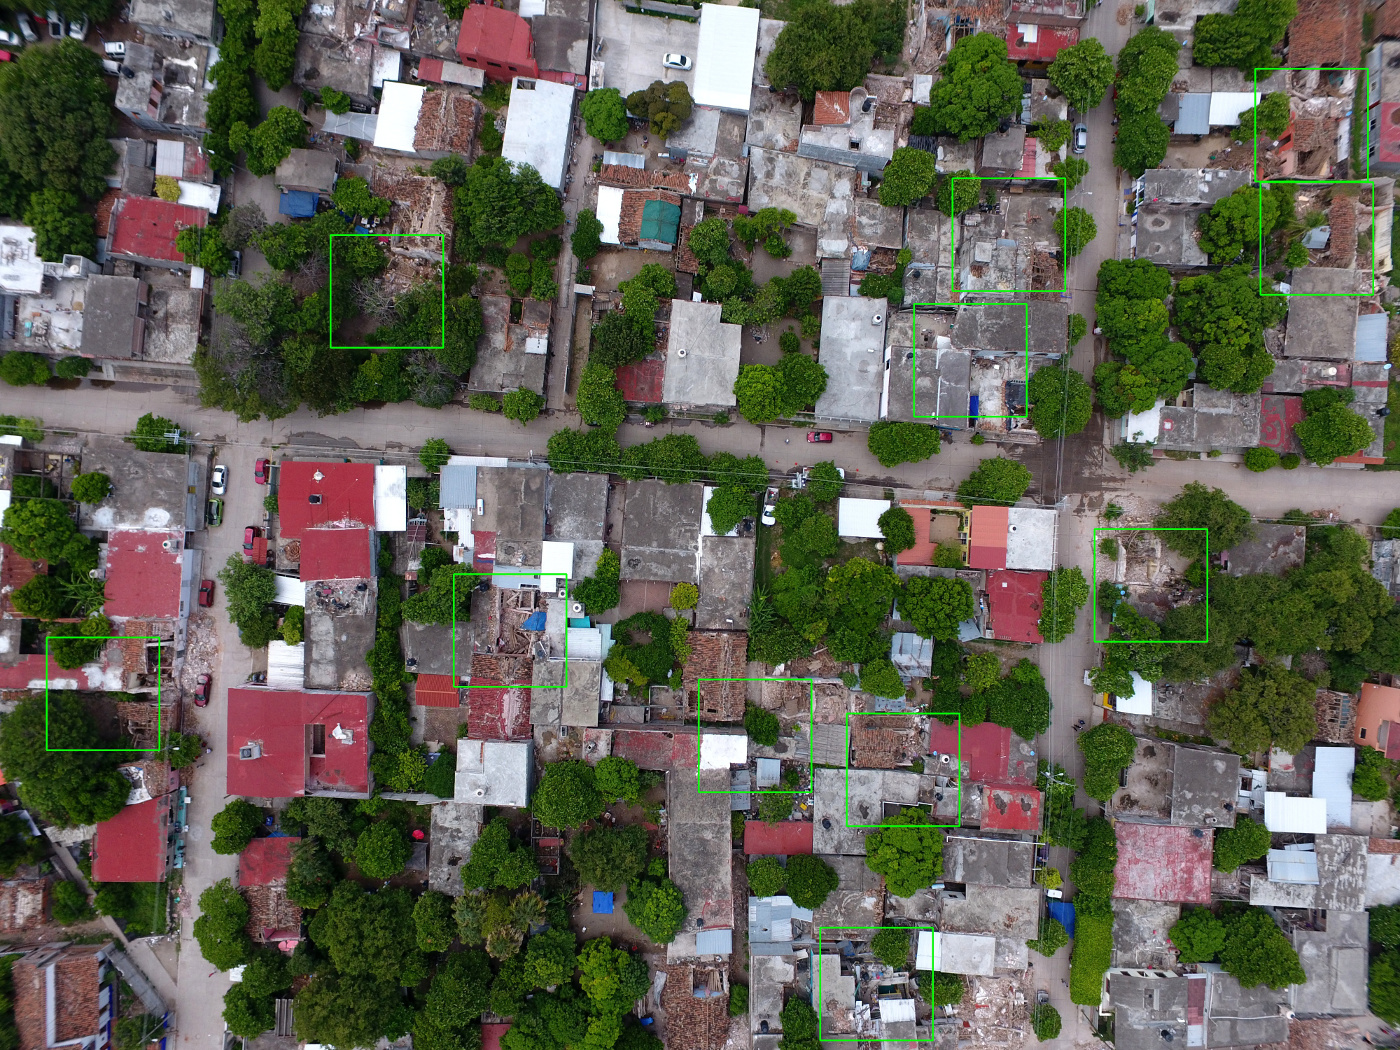
\includegraphics[width=\textwidth]{images/no-overlap.jpg}
  \label{fig:no-overlap}
  \caption{Results of our experiment. As we expected, the graph shows a positive correlation between the accuracy and the number of training samples.}
\end{figure}


\subsection{Orthorectification}

In order to transform our images into useful information from the spatial point of view we need to put them through a process called orthorectification. It removes the effects that arise from the perspective in which the drone took the image. It also stiched and puts the images together to create a mosaic that covers the region of interest. This process needs specialised software, and CENAPRED built those mosaics for us. These rasters are the ones that we use to test our final model. The mosaics gave us the ability to assing coordinates to each of the sites in which the model gave us a positive output. 




\section{Final Results}

Using the methods described in the previous section, we applied our process to the three orthorectified rasters provided by CENAPRED. We randomly placed $322\times322$ pixels boxes along the raster, randomly sampling the location of each of them. The boxes with a positive outcome were saved and post-processed to find overlaps. Once we have the non-overlapping boxes, we transform the center pixel of each box to world coordinates. Finally, these coordinates are used to query Google Maps API obtaining a human-readable address for each point. In table \ref{table:results} we show details of this exercise.\\

We produced a shape-file containing the results for each town given the output of the algorithm. This shape can be overlayed on top of the raster file using a Geographic Information System software such as QGIS. Figures \ref{fig:juchitan-gis},\ref{fig:santamaria-gis}, and \ref{fig:union-gis} show our results. Additionally, the results are also exposed via the REST interface so we can visualize them in the web application as we see in Figure \ref{fig:predict}.\\

\begin{figure}[!h]
  \centering
  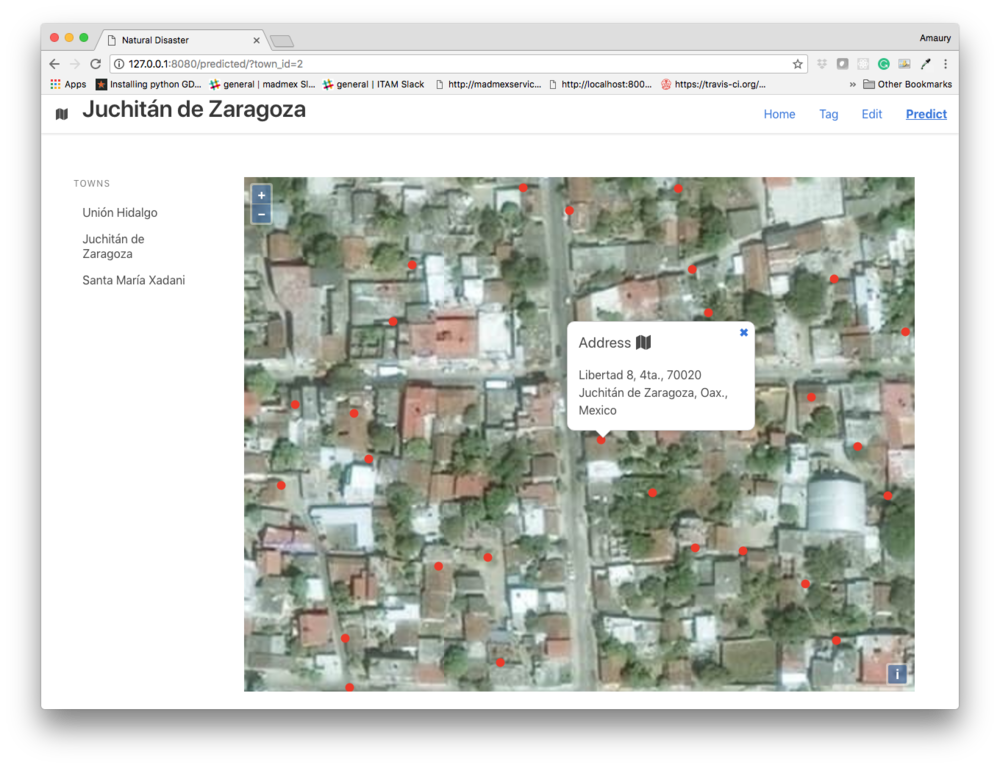
\includegraphics[width=1\textwidth]{images/small-app-predict.png}
  \caption{Predict interface.}
  \label{fig:predict}
\end{figure}


\begin{table}[h!]
  \centering
  \begin{tabular}{|c|c|c|c|c|c|c|c|}
    \hline
    Town                 &Threshold&Positives  & Width & Height & Seconds & Overlap &Windows \\ \hline
    Santa Mar\'ia Xadani   &0.96      &11         & 25598 & 30144  & 16403   & 0.0005  &45704 \\ \hline
    Juchit\'an de Zaragoza &0.96      &562        & 42375 & 28831  & 21216   & 0.0005  &72372 \\ \hline
    Uni\'on Hidalgo        &0.96      &73         & 19945 & 28795  & 11363   & 0.0005  &34188 \\
    \hline
  \end{tabular}
  \caption{We report details on running the algorithm on the orthorectified rasters. Width and height are in pixels. Threshold is our decision boundry to decide wether or not a window is considered to have damage. Windows are the number of predictions that the model gave us. We also report the time in seconds that each process took.}
  \label{table:results}
\end{table}




\begin{figure}[!h]
  \centering
    \begin{subfigure}{.9\textwidth}
        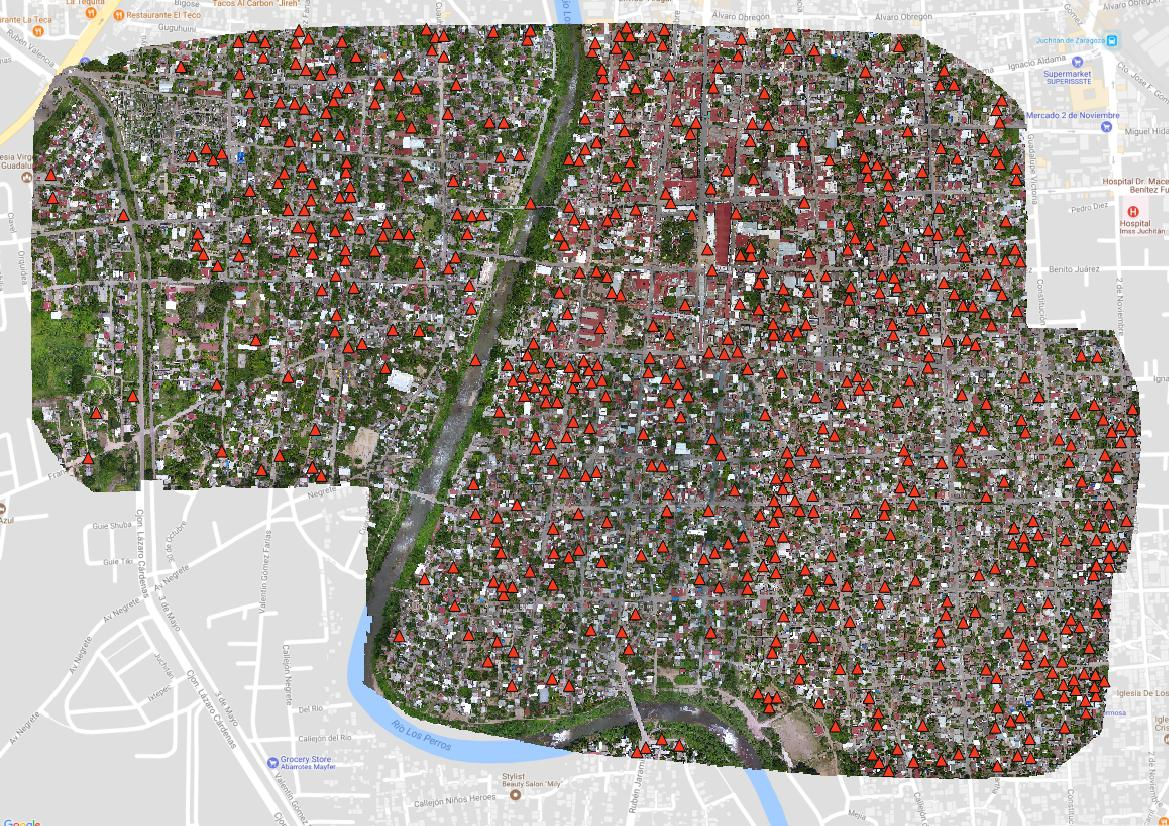
\includegraphics[width=\textwidth]{images/juchitan-ortho.jpg}
    \end{subfigure}
    \begin{subfigure}{.9\textwidth}
        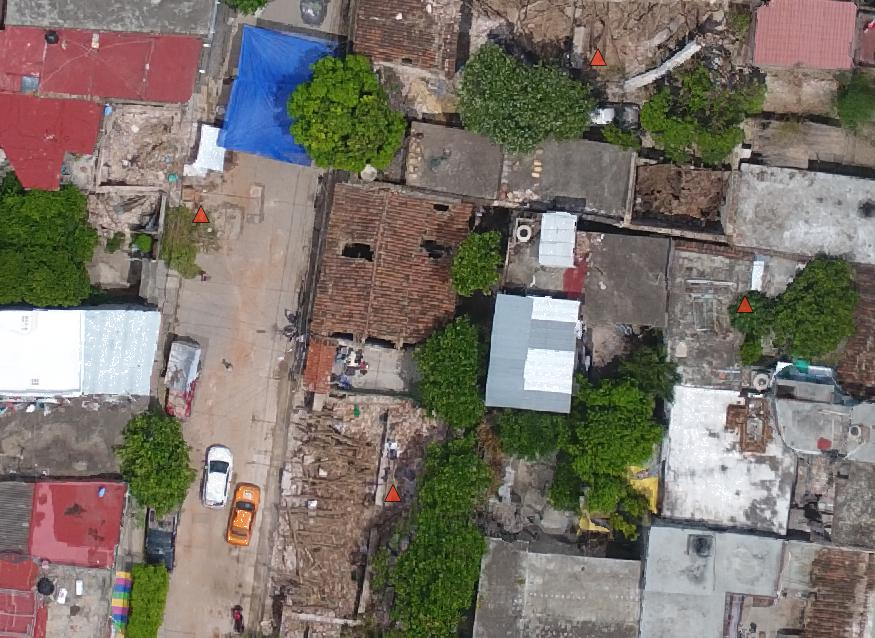
\includegraphics[width=\textwidth]{images/juchitan-example.jpg}
    \end{subfigure}
  \caption{Juchit\'an de Zaragoza.}
  \label{fig:juchitan-gis}
\end{figure}

\begin{figure}[!h]
  \centering
    \begin{subfigure}{.9\textwidth}
        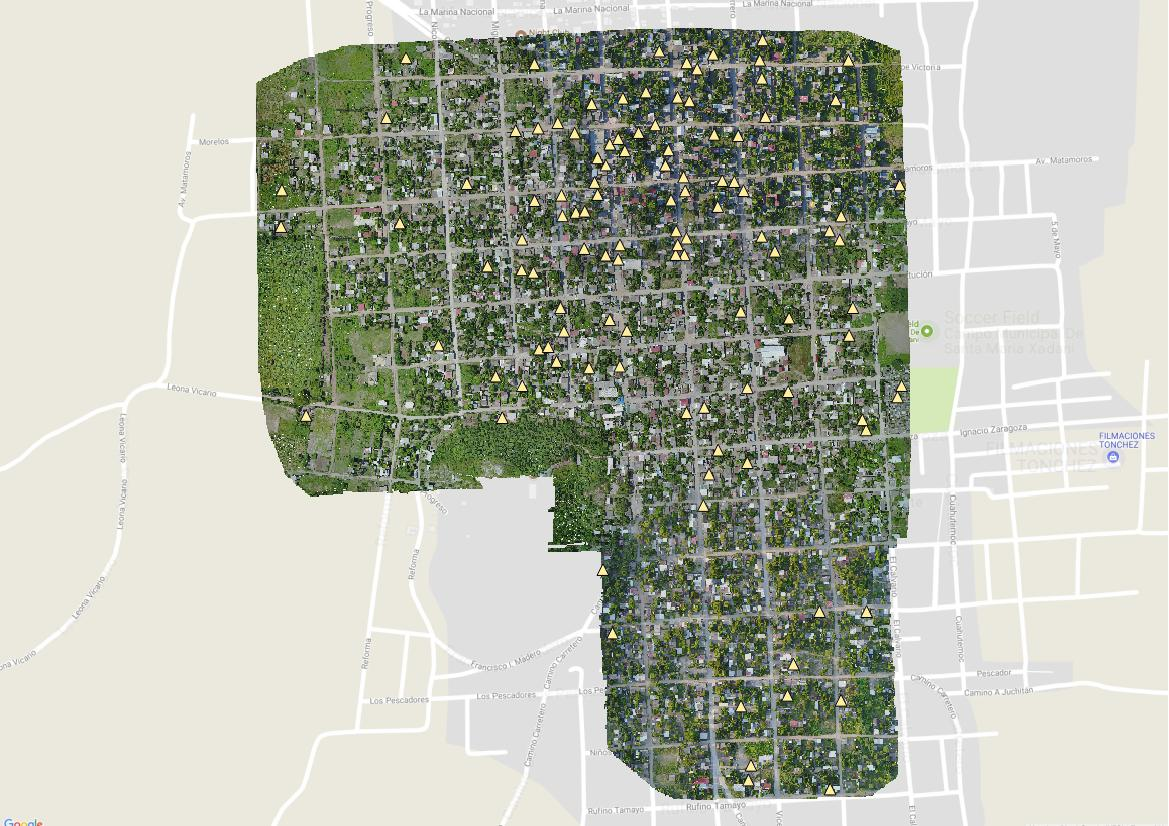
\includegraphics[width=\textwidth]{images/santamaria-ortho.jpg}
    \end{subfigure}
    \begin{subfigure}{.9\textwidth}
        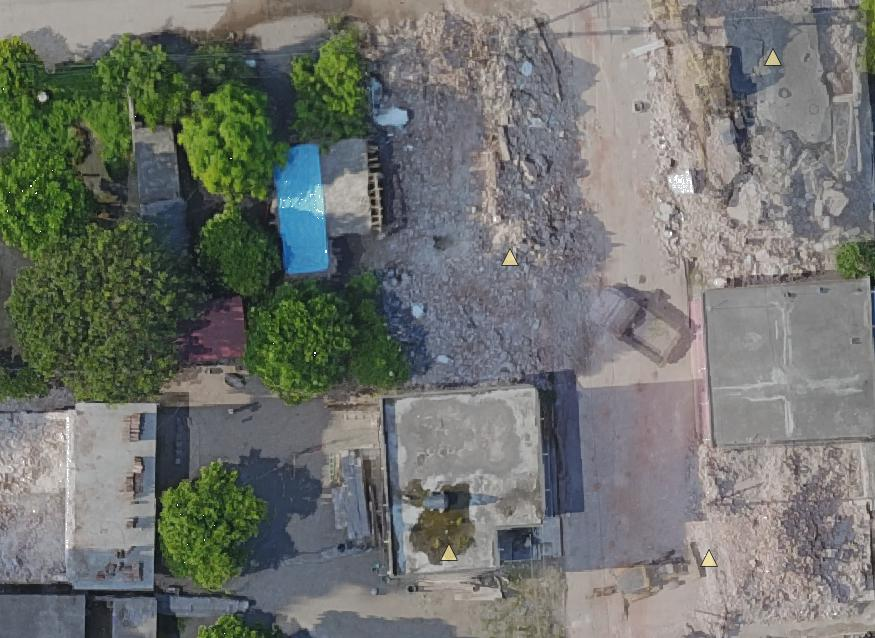
\includegraphics[width=\textwidth]{images/santamaria-example.jpg}
    \end{subfigure}
  \caption{Santa Mar\'ia Xadani.}
  \label{fig:santamaria-gis}
\end{figure}

\begin{figure}[!h]
  \centering
    \begin{subfigure}{.9\textwidth}
        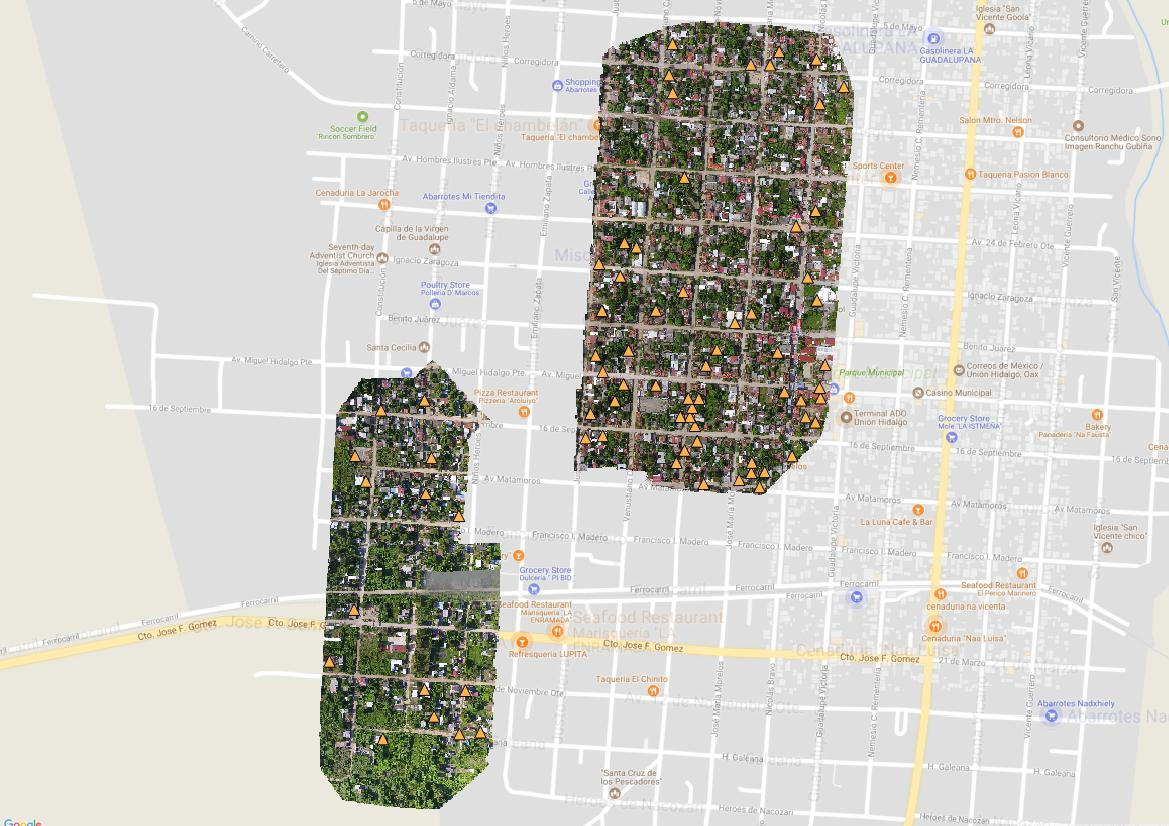
\includegraphics[width=\textwidth]{images/union-ortho.jpg}
    \end{subfigure}
    \begin{subfigure}{.9\textwidth}
        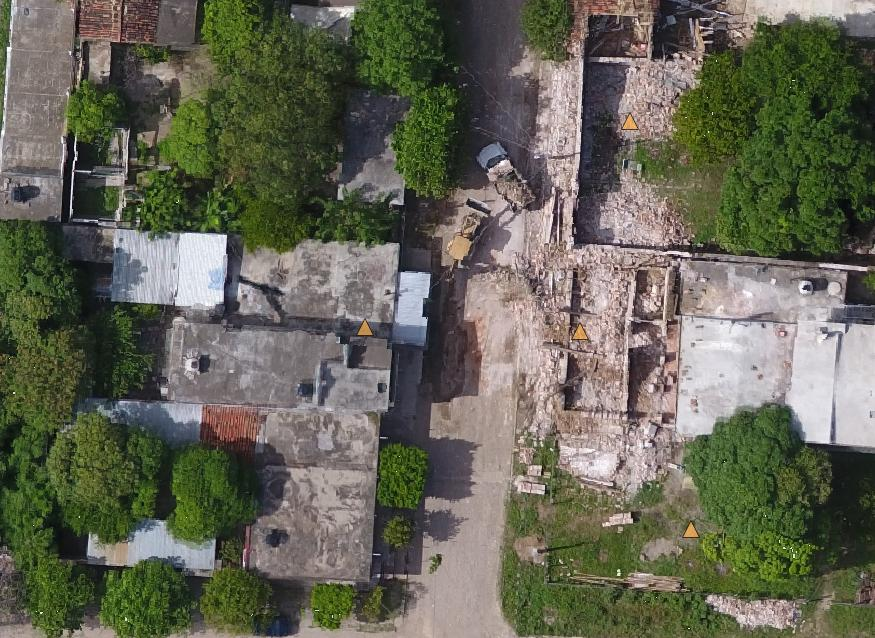
\includegraphics[width=\textwidth]{images/union-example.jpg}
    \end{subfigure}
  \caption{Uni\'on Hidalgo.}
  \label{fig:union-gis}
\end{figure}


